\chapter{Resultados}
\label{cap:resultados}

\section{Alcance de los resultados}

Este capítulo informa identidades analíticas, comparaciones Monte Carlo sobre 13\,500 ejecuciones, una sensibilidad de ingeniería con 40\,500 trayectorias (sección~\ref{sec:engineering-sensitivity}) y una comparación reservada de mapas reducidos afines e híbridos sobre 9\,600 trayectorias (sección~\ref{sec:hybrid-results}). Todas las trayectorias provienen del micromundo especificado sin comisiones. Las corridas y los detalles de reproducción se documentan en el anexo; los identificadores se omiten en la copia anónima.

\section{Resultados analíticos: profundidad e impacto}
\label{sec:res-analitico}

Para una venta fija de $q=500$ unidades de $X$, el impacto $I(q,\kappa x)$ de la ecuación~\eqref{eq:impacto} crece al reducir la reserva (tabla~\ref{tab:impacto}). Con $x=10\,000$, reducir la reserva a la cuarta parte multiplica el impacto por 3.7 y el deslizamiento por 3.5.

\begin{table}[htbp]
\centering
\caption{Impacto de una venta de $q=500$ unidades según la reserva (resultado analítico).}
\label{tab:impacto}
\small
\begin{tabular}{@{}rrrr@{}}
\toprule
Factor de reserva & Reserva $x$ & Impacto $I$ & Deslizamiento (\%) \\
\midrule
1.00 & 10\,000 & 0.09758 & 4.76 \\
0.75 & 7500 & 0.12908 & 6.25 \\
0.50 & 5000 & 0.19062 & 9.09 \\
0.25 & 2500 & 0.36464 & 16.67 \\
\bottomrule
\end{tabular}
\end{table}

La figura~\ref{fig:impacto} muestra la curva completa. Con $I(q,\kappa x)=2\log(1+q/(\kappa x))$ y $\kappa<1$ se cumple $I(q,\kappa x)>I(q,x)$ para todo $q>0$, y la derivada de la ecuación~\eqref{eq:dI} es negativa. Este resultado es una consecuencia algebraica de la regla de producto constante y también sirve como control de la implementación (verificación 8 del anexo).

\subsection{Tasa ideal de corrección con arbitraje acotado}

En ausencia de otras órdenes y con referencia fija, un intercambio limitado a $q=cx$ cambia el precio logarítmico en una magnitud $\delta_c=2\log(1+c)$. Si el error está fuera de la banda, el exceso restante sigue $D_{t+1}=\max(0,D_t-\delta_c)$, y el número ideal de ticks hasta la banda es
\[
  N_\gamma=\left\lceil\frac{D_0}{2\log(1+c)}\right\rceil,\qquad D_0=(|e_0|-\gamma)_+.
\]
Para un choque logarítmico de magnitud $0.20$ y $\gamma=0.003$, se requieren idealmente 20 ticks con $c=0.005$, cuatro con $c=0.03$ y dos con $c=0.10$; con $c=0$ no hay corrección. Por tanto, el resultado de capacidad baja queda en gran medida implicado por la regla y el horizonte de 20 ticks. La simulación aporta información sobre cómo el ruido, la tendencia, el retiro y el orden de eventos alteran ese referente.

\begin{table}[htbp]
\centering
\caption{Corrección idealizada con referencia fija y sin otras órdenes.}
\label{tab:capacity-benchmark}
\small
\begin{tabular}{@{}rrr@{}}
\toprule
Capacidad $c$ & Corrección logarítmica por tick $2\log(1+c)$ & Ticks ideales hasta la banda \\
\midrule
0 & 0 & No hay corrección finita \\
0.005 & 0.00998 & 20 \\
0.03 & 0.05912 & 4 \\
0.10 & 0.19062 & 2 \\
\bottomrule
\end{tabular}
\end{table}

\begin{figure}[htbp]
\centering
\begin{tikzpicture}
\begin{axis}[width=0.78\textwidth,height=6cm,xlabel={Factor de reserva $\kappa$},ylabel={Impacto logarítmico $I$},grid=major,xmin=0.1,xmax=1.05]
\addplot[thick,blue!70!black] table[col sep=comma,x=reserve_factor,y=log_impact] {\datadir/impact_curve.csv};
\end{axis}
\end{tikzpicture}
\caption{Impacto logarítmico de una venta de $q=500$ unidades según el factor de reserva.}
\label{fig:impacto}
\end{figure}

\section{Panorama de las condiciones}

La tabla~\ref{tab:resumen} resume las cinco condiciones, con 2700 ejecuciones cada una (300 semillas por 9 celdas). E1-máx es una extrapolación fuera de los niveles principales de capacidad. Las 300 semillas son una decisión de réplica computacional, no el tamaño de una muestra de mercado.

\begin{table}[htbp]
\centering
\caption{Resumen de las condiciones reservadas (2700 ejecuciones por condición).}
\label{tab:resumen}
\small
\begin{tabular}{@{}lrrrrrr@{}}
\toprule
Condición & Área $A$ & $M$ legado & Recup. & Retorno\,$^{a}$ & Prof. mín. & Retiro \\
\midrule
E0 & 2.363 & 0.1012 & 4.6\,\% & 20.47 & 11667 & 0\,\% \\
E1-baja & 1.056 & 0.1305 & 56.8\,\% & 14.82 & 11667 & 0\,\% \\
E1-alta & 0.100 & 0.1220 & 100.0\,\% & 2.54 & 11667 & 0\,\% \\
E3 & 0.180 & 0.1335 & 96.6\,\% & 4.27 & 6417 & 100\,\% \\
E1-máx & 0.005 & 0.1197 & 100.0\,\% & 1.22 & 11667 & 0\,\% \\
\bottomrule
\multicolumn{7}{@{}l}{\footnotesize $^{a}$ Media restringida con censura en 21 ticks.}
\end{tabular}
\end{table}

El error pico medio es $0.176$ en E0, $0.127$ en E1-baja, $0.064$ en E1-alta, $0.073$ en E3 y $0.008$ en E1-máx. Ninguna orden estuvo limitada por capital en las 13\,500 ejecuciones.

\begin{figure}[htbp]
\centering
\begin{tikzpicture}
\begin{axis}[width=0.9\textwidth,height=6.4cm,xlabel={Tick},ylabel={$|d_t|$ medio},grid=major,legend pos=north east,legend style={font=\scriptsize},xmin=0,xmax=20,ymin=0]
\addplot[thick,red!70!black] table[col sep=comma,x=tick,y=mean_abs_excess,restrict expr to domain={\thisrow{series_id}}{10:10}] {\datadir/trajectories.csv};
\addplot[thick,orange!85!black] table[col sep=comma,x=tick,y=mean_abs_excess,restrict expr to domain={\thisrow{series_id}}{20:20}] {\datadir/trajectories.csv};
\addplot[thick,blue!70!black] table[col sep=comma,x=tick,y=mean_abs_excess,restrict expr to domain={\thisrow{series_id}}{30:30}] {\datadir/trajectories.csv};
\addplot[thick,dashed,green!50!black] table[col sep=comma,x=tick,y=mean_abs_excess,restrict expr to domain={\thisrow{series_id}}{40:40}] {\datadir/trajectories.csv};
\legend{E0,E1-baja,E1-alta,E3}
\end{axis}
\end{tikzpicture}
\caption{Exceso de error medio $|d_t|$ por tick, promediado sobre todas las celdas y semillas.}
\label{fig:trayectorias}
\end{figure}

\section{H1: corrección simulada frente al referente analítico}
\label{sec:res-h1}

El cálculo ideal predice 20 ticks hasta la banda con capacidad baja $c=0.005$, todo el horizonte de simulación; la regla de capacidad alta $c=0.03$ requiere solo cuatro ticks antes de que actúen los demás agentes. En las corridas reservadas, el área de exceso media es $2.363$ en E0, $1.056$ en E1-baja y $0.100$ en E1-alta. La diferencia pareada E1-alta menos E0 es $-2.263$ (mediana $-2.078$; intervalo bootstrap por semilla del 95\,\% $[-2.345,-2.182]$), y los promedios pareados de las 300 semillas son menores con E1-alta. La diferencia E1-alta menos E1-baja es $-0.956$ (intervalo $[-1.003,-0.909]$). Estos valores describen cómo el simulador especificado se aparta del referente simple; la dirección de la corrección por arbitraje se deriva de la propia regla.

\begin{table}[htbp]
\centering
\caption{Resúmenes Monte Carlo pareados (300 semillas). Los intervalos describen variación por semilla bajo el simulador fijo.}
\label{tab:inferencia}
\scriptsize
\setlength{\tabcolsep}{3pt}
\begin{tabularx}{\textwidth}{@{}>{\raggedright\arraybackslash}Xrr>{\raggedright\arraybackslash}p{0.25\textwidth}>{\raggedright\arraybackslash}p{0.16\textwidth}@{}}
\toprule
Contraste & Media $\Delta$ & Mediana & Intervalo 95\,\% & Signo \\
\midrule
H1: área E1-alta menos E0 & $-2.2629$ & $-2.0784$ & $[-2.3448,-2.1820]$ & 100\,\% menor \\
H1: área E1-alta menos E1-baja & $-0.9560$ & $-0.8456$ & $[-1.0034,-0.9091]$ & 100\,\% menor \\
H2: desplazamiento máximo legado & $+0.01143$ & $+0.01140$ & $[0.01074,0.01212]$ & 99.67\,\% mayor \\
H3 mapa menos persistencia, MAE & $-0.000808$ & $-0.000960$ & $[-0.000917,-0.000692]$ & 84.67\,\% menor \\
H3 mapa menos AR(1) escalar, MAE & $+0.0000822$ & $+0.0000844$ & $[0.0000780,0.0000864]$ & 97.67\,\% mayor \\
\bottomrule
\end{tabularx}
\end{table}

\subsection{Tasa de recuperación}

La recuperación sostenida depende de la capacidad y de la celda (tabla~\ref{tab:recuperacion}). Sin arbitraje apenas ocurre. Con capacidad baja varía entre 20 y 100\,\%, y es más baja cuanto mayor es el choque: un choque grande exige más pasos acotados por $c\,x$. Con capacidad alta y máxima es total en todas las celdas.

\begin{table}[htbp]
\centering
\caption{Tasa de recuperación sostenida (\%) por celda y condición.}
\label{tab:recuperacion}
\small
\begin{tabular}{@{}rrrrrrr@{}}
\toprule
$\kappa$ & Choque & E0 & E1-baja & E1-alta & E3 & E1-máx \\
\midrule
0.5 & $-0.05$ & 21.7 & 54.7 & 100.0 & 87.0 & 100.0 \\
0.5 & $-0.10$ & 1.3 & 45.3 & 100.0 & 86.7 & 100.0 \\
0.5 & $-0.20$ & 5.3 & 29.3 & 100.0 & 95.7 & 100.0 \\
1 & $-0.05$ & 0.0 & 72.0 & 100.0 & 100.0 & 100.0 \\
1 & $-0.10$ & 3.7 & 59.3 & 100.0 & 100.0 & 100.0 \\
1 & $-0.20$ & 0.0 & 20.3 & 100.0 & 100.0 & 100.0 \\
2 & $-0.05$ & 9.7 & 100.0 & 100.0 & 100.0 & 100.0 \\
2 & $-0.10$ & 0.0 & 99.0 & 100.0 & 100.0 & 100.0 \\
2 & $-0.20$ & 0.0 & 31.0 & 100.0 & 100.0 & 100.0 \\
\bottomrule
\end{tabular}
\end{table}

La tabla~\ref{tab:h1-ideal-times} compara las tasas de retorno simulado al plazo predicho por el referente de piscina aislada con las tasas al horizonte completo de 20 ticks. La primera tasa no representa el evento de primera entrada del referente: la recuperación simulada exige dos observaciones posarbitraje consecutivas dentro de la banda y registra el tick inicial de ese par. La tabla alinea el plazo y conserva el criterio más exigente de retorno sostenido. Cada celda contiene 300 semillas; el CSV reproducible incluye intervalos de Wilson.

\begin{table}[htbp]
\centering
\caption{Tasas de retorno sostenido simulado al plazo ideal de primera entrada y al tick 20. Cada valor indica porcentaje por $N_\gamma$ / porcentaje al tick 20 ($n=300$).}
\label{tab:h1-ideal-times}
\scriptsize
\setlength{\tabcolsep}{4pt}
\begin{tabularx}{\textwidth}{@{}rrr>{\centering\arraybackslash}X>{\centering\arraybackslash}X@{}}
\toprule
Profundidad $\kappa$ & Choque & $N_\gamma$ ($c=.005/.03$) & $c=.005$ & $c=.03$ \\
\midrule
0.5 & $-0.05$ & 5 / 1 & 17.7 / 54.7 & 49.0 / 100.0 \\
1.0 & $-0.05$ & 5 / 1 & 21.3 / 72.0 & 57.3 / 100.0 \\
2.0 & $-0.05$ & 5 / 1 & 43.7 / 100.0 & 100.0 / 100.0 \\
0.5 & $-0.10$ & 10 / 2 & 28.3 / 45.3 & 59.3 / 100.0 \\
1.0 & $-0.10$ & 10 / 2 & 28.7 / 59.3 & 83.3 / 100.0 \\
2.0 & $-0.10$ & 10 / 2 & 44.7 / 99.0 & 100.0 / 100.0 \\
0.5 & $-0.20$ & 20 / 4 & 29.3 / 29.3 & 84.0 / 100.0 \\
1.0 & $-0.20$ & 20 / 4 & 20.3 / 20.3 & 79.7 / 100.0 \\
2.0 & $-0.20$ & 20 / 4 & 31.0 / 31.0 & 98.3 / 100.0 \\
\bottomrule
\end{tabularx}
\end{table}

La tabla también muestra cuándo el referente aislado es informativo y cuándo importan las interacciones. Con capacidad $c=0.03$ y factor de profundidad $\kappa=2$, el 100\,\% de las trayectorias satisface el criterio de retorno sostenido antes del plazo ideal para los choques $-0.05$ y $-0.10$, y el 98.3\,\% lo hace para $-0.20$. Con $\kappa=0.5$ y $1$, solo el 49.0--84.0\,\% y el 57.3--83.3\,\%, respectivamente, lo logra antes de ese plazo, aunque todas las trayectorias con $c=0.03$ se recuperan antes del tick 20. La diferencia refleja las órdenes continuas y el orden de eventos del calendario simulado; no contradice el límite de piscina aislada, cuyos supuestos excluyen esos mecanismos. La simulación cumple así una función acotada: cuantificar las desviaciones en horizonte finito frente a un referente mecánico.

\subsection{Desglose por celda}

El efecto de H1 es negativo en todas las celdas (tabla~\ref{tab:celdas}); su magnitud crece con el choque, porque sin arbitraje el exceso se acumula durante los 20 ticks. La heterogeneidad entre semillas es grande (figura~\ref{fig:cuantiles}): el contraste va de $-4.60$ a $-1.38$.

\begin{table}[htbp]
\centering
\caption{Diferencia media por celda de los contrastes H1 (primario y de capacidad) y H2.}
\label{tab:celdas}
\small
\begin{tabular}{@{}rrrrrc@{}}
\toprule
$\kappa$ & Choque & E1-alta vs. E0 & E1-alta vs. E1-baja & Diferencia en $M$ legado & Reservada \\
\midrule
0.5 & $-0.05$ & $-1.630$ & $-0.832$ & $+0.0523$ & sí \\
0.5 & $-0.10$ & $-1.873$ & $-0.941$ & $+0.0361$ & sí \\
0.5 & $-0.20$ & $-3.128$ & $-1.703$ & $+0.0146$ & sí \\
1 & $-0.05$ & $-1.222$ & $-0.294$ & $0.0000$ & sí \\
1 & $-0.10$ & $-2.023$ & $-0.652$ & $0.0000$ & no \\
1 & $-0.20$ & $-3.784$ & $-1.883$ & $0.0000$ & sí \\
2 & $-0.05$ & $-1.007$ & $-0.116$ & $0.0000$ & sí \\
2 & $-0.10$ & $-1.951$ & $-0.450$ & $0.0000$ & sí \\
2 & $-0.20$ & $-3.748$ & $-1.732$ & $0.0000$ & sí \\
\bottomrule
\end{tabular}
\end{table}

\begin{figure}[htbp]
\centering
\begin{tikzpicture}
\begin{axis}[width=0.8\textwidth,height=6cm,xlabel={Cuantil},ylabel={Contraste por semilla},grid=major,legend pos=south east,legend style={font=\scriptsize}]
\addplot[thick,blue!70!black,mark=*,mark size=1.5pt] table[col sep=comma,x=quantile,y=value,restrict expr to domain={\thisrow{contrast_id}}{1:1}] {\datadir/delta_quantiles.csv};
\addplot[thick,orange!85!black,mark=square*,mark size=1.5pt] table[col sep=comma,x=quantile,y=value,restrict expr to domain={\thisrow{contrast_id}}{2:2}] {\datadir/delta_quantiles.csv};
\legend{H1 primario,H1 capacidad}
\end{axis}
\end{tikzpicture}
\caption{Cuantiles del contraste por semilla de H1 ($\Delta_1$ y comparación de capacidades).}
\label{fig:cuantiles}
\end{figure}

\section{H2: sensibilidad al retiro y a la escala de las órdenes}
\label{sec:res-h2}

Con el estadístico legado $M=\max_t|\log(p_t^D/p_0^D)|$, la diferencia pareada E3 menos E1-alta es $+0.0114$ en promedio (intervalo bootstrap por semilla del 95\,\% $[0.0107,0.0121]$). Este estadístico mide el desplazamiento respecto del precio del AMM previo al choque, no el sobrepaso ni el error máximo de seguimiento respecto de la nueva referencia CEX. Además, se satura en $|\text{choque}|+\gamma$ en seis de nueve celdas. Se conserva solo como descripción del diseño original. El máximo de horizonte completo $P=\max_{0\le t\le20}|e_t|$ tiene una limitación relacionada: incluye el tick 1, cuando el choque impuesto domina ambas condiciones, por lo que su contraste disminuye al crecer el choque.

Las diferencias por celda de la tabla~\ref{tab:celdas} son positivas solo con factor de profundidad $\kappa=0.5$ y nulas con $\kappa=1$ y $2$. El retiro se activa en todas las trayectorias E3 porque cada choque aplicado supera el umbral fijo $|e_t|>0.02$; normalmente ocurre en el tick 1. Esto es una intervención determinista única bajo los choques ensayados, no una prueba de respuestas heterogéneas o graduales. La orden de pánico se activa solo con $\kappa=0.5$, donde el impacto configurado de la orden de ruido es 1.6\,\%, apenas 0.1 puntos porcentuales por encima del umbral de 1.5\,\%.

Por ello, repetimos las trayectorias con semillas archivadas y usamos como diagnóstico exploratorio H2 principal el exceso de error acumulado después de confirmar la recuperación. Sea $t_c$ el segundo de dos ticks consecutivos dentro de la banda que definen el retorno sostenido; entonces $A_{\mathrm{post}}=\sum_{t>t_c}(|e_t|-\gamma)_+$. Con profundidad $\kappa=0.5$, la diferencia pareada E3 menos E1-alta es $0.1229$ (intervalo bootstrap por semilla del 95\,\% $[0.1092,0.1373]$, $n=267$), $0.1239$ ($[0.1134,0.1348]$, $n=272$) y $0.1215$ ($[0.1109,0.1326]$, $n=287$) para choques de $-0.05$, $-0.10$ y $-0.20$, respectivamente. Con profundidades 1 y 2, los contrastes pareados son cero a precisión numérica en todas las celdas de choque. La figura~\ref{fig:h2-post-recovery} muestra este patrón por profundidad. La similitud de los contrastes de baja profundidad entre los tamaños de choque, tras excluir el choque y los dos ticks de confirmación, es más pertinente para estudiar la fragilidad posterior al retorno que la métrica pico anterior. Sigue siendo una comparación posterior al análisis inicial y condicionada a trayectorias recuperadas, no un efecto confirmatorio ni de mercado.

\begin{figure}[htbp]
\centering
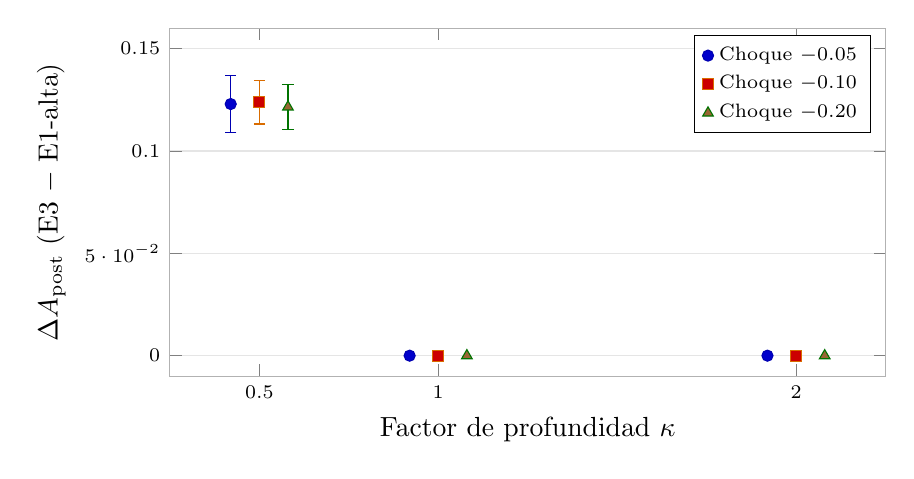
\begin{tikzpicture}
\begin{axis}[
  width=0.88\textwidth,height=6.0cm,
  xlabel={Factor de profundidad $\kappa$}, ylabel={$\Delta A_{\mathrm{post}}$ (E3 $-$ E1-alta)},
  xmin=0.25,xmax=2.25,ymin=-0.01,ymax=0.16,
  xtick={0.5,1,2}, ymajorgrids=true, grid style={gray!20},
  legend style={font=\scriptsize,at={(0.98,0.98)},anchor=north east},
  axis line style={gray!60}, tick label style={font=\scriptsize}
]
\addplot+[only marks,mark=*,mark size=2pt,blue!70!black,error bars/.cd,y dir=both,y explicit] coordinates {
  (0.42,0.12295) +- (0,0.01402) (0.92,0) (1.92,0)
};
\addlegendentry{Choque $-0.05$}
\addplot+[only marks,mark=square*,mark size=2pt,orange!85!black,error bars/.cd,y dir=both,y explicit] coordinates {
  (0.50,0.12393) +- (0,0.01071) (1.00,0) (2.00,0)
};
\addlegendentry{Choque $-0.10$}
\addplot+[only marks,mark=triangle*,mark size=2.2pt,green!45!black,error bars/.cd,y dir=both,y explicit] coordinates {
  (0.58,0.12154) +- (0,0.01083) (1.08,0) (2.08,0)
};
\addlegendentry{Choque $-0.20$}
\end{axis}
\end{tikzpicture}
\caption{Contraste del área de exceso posterior a la recuperación según la profundidad probada. Las barras aproximan de forma simétrica los intervalos bootstrap pareados del 95\,\% con $\kappa=0.5$; los contrastes con $\kappa=1$ y $2$ son cero a precisión numérica. En baja profundidad, los tamaños pareados son 267, 272 y 287; las tres profundidades usan 300 semillas archivadas.}
\label{fig:h2-post-recovery}
\end{figure}

El contraejemplo de la razón de presión se puede interpretar mecánicamente dentro del diseño ensayado. Con profundidad baja y capacidad $c=0.03$, el flujo continuo configurado de ruido más tendencia produce $R_{\mathrm{flow}}=0.670$ en el caso estático, por debajo de uno; la orden de pánico única produce $R_{\mathrm{panic}}=1.327$, y el flujo adverso máximo configurado de ruido más pánico da $R_{\max}^{\mathrm{adv}}=1.586$. En la reserva nominal de E3 tras el retiro, las razones son 1.208, 2.375 y 2.831 (tabla~\ref{tab:pressure-ratio}). La repetición sin pánico no muestra salidas posteriores en E1-alta estático (0/300 para cada choque; límite superior Wilson del 95\,\% de 1.3\,\%), mientras que las salidas con pánico permitido son episodios únicos y las 143 coinciden con el tick de la orden de pánico. En E3, el 98.2--99.6\,\% de las trayectorias recuperadas vuelve a salir, y la mayoría presenta episodios múltiples. Este patrón se mantiene al desactivar el pánico. En estas celdas, la evidencia respalda una salida única asociada al pánico para E1 y salidas recurrentes bajo E3 que no requieren pánico. No establece umbrales universales: las razones usan órdenes configuradas y reservas aproximadas, no flujo direccional realizado en cada evento.

El control pareado de referencia de capacidad con $\kappa=0.5$ fija el límite de entrada del arbitraje en $c$ por la reserva inicial, mientras la ejecución sigue limitada por las reservas activas. Sus razones con límite fijo coinciden con las de E1 estático ($R_{\mathrm{flow}}\approx0.67$, $R_{\mathrm{panic}}\approx1.32$), y el contraste del área posrecuperación disminuye de 0.122--0.124 a 0.0036--0.0097, como predice $R$. Esto no descompone efectos independientes de capacidad y profundidad: ambas son componentes de la misma razón orden/reserva. Como las E3 que no se recuperan quedan fuera del contraste condicional, la estimación puede subestimar la fragilidad sobre todas las trayectorias. El diseño factorial más amplio que varíe retiro, capacidad y profundidad sigue siendo necesario.



El seguimiento amplio requiere un diseño factorial prerregistrado que varíe por separado retiro, referencia de capacidad, profundidad, escala de órdenes y pánico. El replay actual es exploratorio y reutiliza semillas existentes; no aporta una muestra independiente.

\section{H3: comparación predictiva con referencias simples}
\label{sec:res-h3}

La cláusula del mapa se responde aquí comparando la descripción predictiva del error continuo en trayectorias reservadas del simulador; las etiquetas de horizonte finito son resúmenes descriptivos, no clases observadas. El mapa de dos estados se ajusta al exceso de error con signo $d_t$, que vale cero dentro de la banda y cambia de pendiente en su límite. Una sola relación afín no puede representar exactamente este umbral. En celdas reservadas, el mapa tiene menor error absoluto medio que la persistencia en la mayoría de condiciones, pero no supera al AR(1) escalar en ninguna condición principal. Por tanto, su segundo estado no demuestra valor predictivo incremental a un paso en este diseño; el mapa queda como resumen descriptivo del simulador, no como modelo de regímenes.

\begin{table}[htbp]
\centering
\caption{Error absoluto medio a un paso en celdas reservadas del simulador.}
\label{tab:h3}
\small
\begin{tabular}{@{}lrrrc@{}}
\toprule
Condición & Mapa dos estados & Persistencia & AR(1) escalar & Mapa mejora persistencia \\
\midrule
E0 & 0.01765 & 0.01751 & 0.01757 & no \\
E1-baja & 0.01573 & 0.01615 & 0.01566 & sí \\
E1-alta & 0.00493 & 0.00620 & 0.00486 & sí \\
E3 & 0.00929 & 0.01096 & 0.00916 & sí \\
E1-máx$^{\ast}$ & 0.00567 & 0.00594 & 0.00578 & sí \\
\bottomrule
\multicolumn{5}{@{}l}{\footnotesize $^{\ast}$ Condición de extrapolación fuera de los niveles principales de capacidad.}
\end{tabular}
\end{table}

Promediada sobre las cuatro condiciones principales, la diferencia mapa menos persistencia es $-0.000808$ (intervalo bootstrap por semilla del 95\,\% $[-0.000917,-0.000692]$); la diferencia mapa menos AR escalar es $+0.0000822$ (intervalo $[0.0000780,0.0000864]$). Estos intervalos describen variación Monte Carlo. Las etiquetas de trayectorias finitas resumen las mismas corridas y no son regímenes observados de forma independiente.

\section{Comparación reservada de mapas afines e híbridos}
\label{sec:hybrid-results}

La nueva comparación usa el análisis 0.1.0, ejecución \code{\HybridRunID} y el error de precio con signo. En 9\,600 trayectorias reservadas de 300 semillas nuevas, el mapa híbrido redujo el MAE recursivo medio del error de precio de 0.030807 a 0.030291. La mejora pareada media fue 0.000516 (intervalo bootstrap por semilla del 95\,\% [0.000499, 0.000533]); el 99.7\,\% de los contrastes promediados por semilla favoreció a Hyb. La mejora media frente a L0 es de aproximadamente 1.7\,\%. Es una pequeña ganancia en error de reproducción dentro del simulador especificado; la evaluación recibe la trayectoria futura realizada del CEX y no constituye un pronóstico en tiempo real.

Cada condición aportó 12\,000 transiciones de selección. Hubo observaciones a ambos lados de la banda (tabla~\ref{tab:hybrid-regimes}), aunque el modelo de arbitraje bajo tuvo menos observaciones dentro de ella. El ajuste sigue siendo específico para cada condición, y estos conteos no demuestran que las dos variables de estado capturen toda la memoria relevante para la transición.

\begin{table}[htbp]
\centering
\caption{Transiciones de selección dentro y fuera de la banda configurada.}
\label{tab:hybrid-regimes}
\small
\begin{tabular}{@{}lrrr@{}}
\toprule
Condición & En banda & Fuera de banda & Total \\
\midrule
E0 & 681 & 11\,319 & 12\,000 \\
E1-baja & 1\,466 & 10\,534 & 12\,000 \\
E1-alta & 3\,776 & 8\,224 & 12\,000 \\
E3 & 2\,834 & 9\,166 & 12\,000 \\
\bottomrule
\end{tabular}
\end{table}

La mejora no se distribuye entre las condiciones operativas. Se concentra en el arbitraje de capacidad baja, especialmente con profundidad 2, donde la ganancia promediada entre los cuatro choques reservados es 0.003943. Con profundidad 0.5, la ganancia correspondiente es 0.000354. Los promedios de las demás combinaciones de condición y profundidad se encuentran entre aproximadamente $-0.000101$ y $-0.000002$, lo que favorece levemente a L0. El MAE secundario a un paso para $e$ mejora de 0.014882 a 0.014800, mientras que los errores a un paso y recursivos de la presión de flujo $z$ son ligeramente peores con Hyb. Por tanto, el resultado respalda una ventaja limitada y dependiente de la condición de los términos de banda para predecir el error de precio; no muestra una superioridad uniforme del mapa híbrido ni que las variables de estado representen todo el proceso.

\begin{figure}[H]
\centering
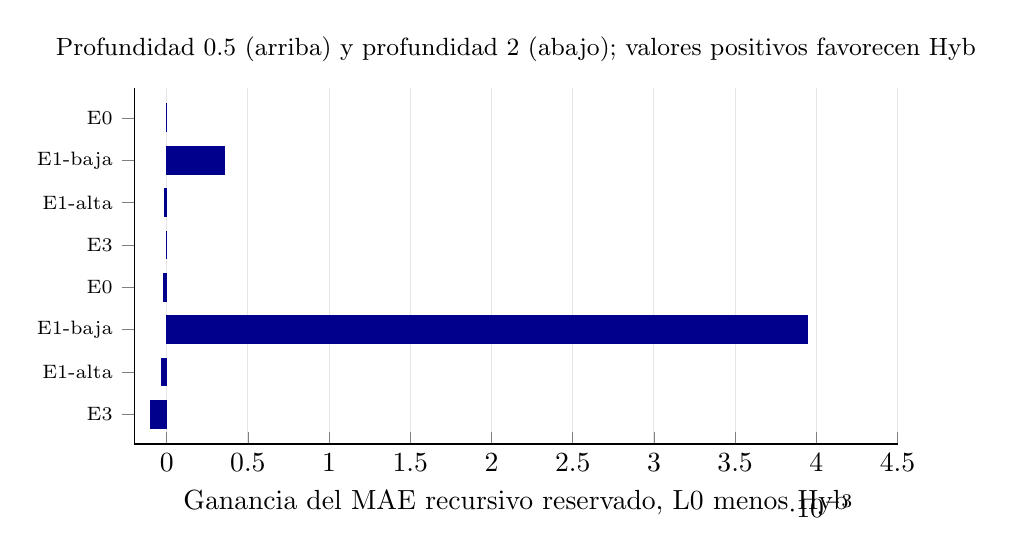
\begin{tikzpicture}
\begin{axis}[
  xbar, width=0.93\textwidth, height=6.1cm,
  xmin=-0.0002, xmax=0.0045,
  xlabel={Ganancia del MAE recursivo reservado, L0 menos Hyb},
  symbolic y coords={C1,C2,C3,C4,C5,C6,C7,C8}, ytick=data,
  yticklabels={E0, E1-baja, E1-alta, E3, E0, E1-baja, E1-alta, E3},
  yticklabel style={font=\scriptsize},
  y dir=reverse, xmajorgrids=true, grid style={gray!20},
  axis x line*=bottom, axis y line*=left,
  title style={font=\small}, title={Profundidad 0.5 (arriba) y profundidad 2 (abajo); valores positivos favorecen Hyb}
]
\addplot[fill=blue!55!black,draw=blue!55!black] coordinates {
  (-0.000002,C1) (0.000354,C2) (-0.000014,C3) (-0.000003,C4)
  (-0.000017,C5) (0.003943,C6) (-0.000033,C7) (-0.000101,C8)
};
\end{axis}
\end{tikzpicture}
\caption{Ganancia media del MAE recursivo del error de precio por condición operativa y profundidad. Cada barra promedia cuatro magnitudes de choque reservadas; los contrastes por celda son descriptivos y no tienen intervalos de confianza separados. Los valores se exportan en \code{figures/data/hybrid\_depth\_condition.csv}.}
\label{fig:hybrid-cell-gains}
\end{figure}

La ganancia media del mapa híbrido no debe interpretarse aisladamente: casi toda la ganancia proviene de una combinación de baja capacidad y profundidad, mientras que la predicción de la presión de flujo no mejora. El siguiente paso de modelado consiste en representar explícitamente los límites de capacidad y las transiciones de retiro de LP y evaluarlos con otro protocolo congelado, en vez de añadir más términos polinómicos libres. La comparación de mapas es un diagnóstico de reproducción dentro del simulador, no un pronóstico de mercado ni una afirmación de estabilidad del sistema completo.

\section{Trayectorias por profundidad}

La figura~\ref{fig:prof} compara E1-alta y E3 con $\kappa=0.5$. Con la menor profundidad, E3 parte del mismo exceso inicial y se corrige más despacio. Una explicación compatible es que el retiro reduce tanto la profundidad como el límite de arbitraje $c\,x$; estos mecanismos están acoplados en el diseño actual. Con $\kappa=1$ y $2$ las dos trayectorias son casi idénticas. El retorno sostenido ocurre en promedio en el tick $7.8$ para E3 con $\kappa=0.5$ frente a $2.8$ para E1-alta, mientras que con $\kappa=1$ y $2$ las diferencias son de $0.1$ ticks o menos.

\begin{figure}[htbp]
\centering
\begin{tikzpicture}
\begin{axis}[width=0.9\textwidth,height=6.2cm,xlabel={Tick},ylabel={$|d_t|$ medio},grid=major,legend style={font=\scriptsize},xmin=0,xmax=20,ymin=0]
\addplot[thick,blue!70!black] table[col sep=comma,x=tick,y=mean_abs_excess,restrict expr to domain={\thisrow{series_id}}{31:31}] {\datadir/trajectories.csv};
\addplot[thick,dashed,green!50!black] table[col sep=comma,x=tick,y=mean_abs_excess,restrict expr to domain={\thisrow{series_id}}{41:41}] {\datadir/trajectories.csv};
\legend{E1-alta,E3}
\end{axis}
\end{tikzpicture}
\caption{Exceso de error medio con $\kappa=0.5$: arbitraje alto estático (E1-alta) y con retiro por umbral (E3).}
\label{fig:prof}
\end{figure}

\section{Sensibilidad de ingeniería: recuperación y escala de las órdenes}
\label{sec:engineering-sensitivity}

Un análisis suplementario (análisis 0.6.0, ejecución \code{\EngineeringRunID}) usó 300 semillas nuevas (2000--2299), tres variantes de flujo de órdenes y las 15 celdas de profundidad/choque/condición de la grilla de diseño reservada: 40\,500 trayectorias de 20 ticks abstractos. Es un análisis descriptivo y exploratorio de sensibilidad, no un contraste inferencial. La recuperación significa el primer par observado de ticks consecutivos dentro de la banda; las salidas posteriores se contabilizan por separado. Los plazos se expresan en ticks, no en tiempo transcurrido.

Con los tamaños absolutos originales, E3 con retiro por umbral se recuperó al menos una vez en el 97.4\,\% de las trayectorias, pero solo el 81.9\,\% terminó dentro de la banda. De las trayectorias que se recuperaron, el 31.2\,\% salió después. Con profundidad 0.5, solo el 45.8\,\% terminó dentro de la banda y el 98.8\,\% de las trayectorias recuperadas salió posteriormente. Por tanto, en este modelo, un primer retorno sostenido no equivale a un seguimiento persistente. Estos promedios igualmente ponderados del diseño no sustentan una afirmación poblacional con ajuste por multiplicidad.

El contraste de respuesta máxima entre E3 con retiro por umbral y estático cambia según la definición de las órdenes (tabla~\ref{tab:engineering-sensitivity}). Mantener fijos los tamaños absolutos produjo un efecto con profundidad 0.5; al escalar las órdenes de ruido y tendencia con las reservas iniciales, el contraste fue efectivamente cero en las tres profundidades. Desactivar el pánico redujo, pero no eliminó, esta métrica de horizonte completo dominada por el choque. El análisis posterior a la recuperación que sigue separa ese evento único de las salidas posteriores. Esta sensibilidad muestra que la profundidad por sí sola no determina el resultado; también importan el tamaño de la orden relativo a las reservas y la regla de reacción.

\begin{table}[htbp]
\centering
\caption{Respuesta máxima suplementaria pareada: E3 con retiro por umbral menos estático por profundidad (300 semillas nuevas). Intervalos aproximados del 95\,\% sin ajuste.}
\label{tab:engineering-sensitivity}
\small
\begin{tabular}{@{}lrrr@{}}
\toprule
Variante del flujo de órdenes & Profundidad 0.5 & Profundidad 1 & Profundidad 2 \\
\midrule
Órdenes absolutas fijas & 0.03458 [0.03225, 0.03690] & 0.00000 & 0.00000 \\
Órdenes proporcionales a reservas iniciales & 0.00000 & 0.00000 & 0.00000 \\
Órdenes fijas, sin pánico & 0.01471 [0.01364, 0.01577] & 0.00000 & 0.00000 \\
\bottomrule
\end{tabular}
\end{table}

Con profundidad 0.5 y órdenes absolutas fijas, E3 con retiro por umbral terminó dentro de la banda en el 45.8\,\% de las trayectorias; con órdenes proporcionales, terminó dentro en el 100\,\%. Estas variantes comparten el mismo modelo estilizado de agentes representativos y no constituyen comparaciones empíricas. Los resúmenes por celda, contrastes pareados, configuración y hashes completos se exportan en \code{figures/engineering/}.

\subsection{Presión y mecanismos de salida: repetición exploratoria}

El protocolo exploratorio congelado 0.7.0 repite 9\,000 trayectorias con semillas existentes 2000--2299: 5\,400 con órdenes fijas en las tres profundidades y choques, 1\,800 trayectorias poco profundas sin pánico y 1\,800 trayectorias poco profundas con el límite de entrada del arbitraje fijado a su valor basado en reservas iniciales. Las 7\,200 trayectorias con el límite ligado a las reservas originales reproducen exactamente las métricas archivadas de recuperación, salidas, área de exceso, respuesta máxima y límites de capital. Es un análisis de reproducibilidad y mecanismos con semillas existentes, no una muestra Monte Carlo independiente.

Para una orden configurada $q$ y reserva $x$, definimos $R(q,x,c)=2\log(1+q/x)/\delta_c$, donde $\delta_c=2\log(1+c)$. El diagnóstico conservador de un tick es $R_{\mathrm{1tick}}=\max_{q\in\mathcal Q_{\mathrm{adv}}}R(q,x,c)$, donde $\mathcal Q_{\mathrm{adv}}$ incluye la mayor entrada adversa configurada, incluido el pánico. Con profundidad 0.5 y capacidad $c=0.03$, el desglose informa $R_{\mathrm{flow}}$ para $q=100$ (ruido y tendencia alineados), $R_{\mathrm{panic}}$ para la orden única de pánico $q=200$, y $R_{\mathrm{1tick}}=R_{\max}^{\mathrm{adv}}$ para $q=240$ (ruido y pánico alineados; el pánico sustituye a la tendencia, no se suma a ella). Para E3, la reserva posterior al retiro se aproxima como el 55\,\% de la inicial. Son razones configuradas, no mediciones de flujo por tick: el ruido ocurre con probabilidad 0.7, las direcciones pueden diferir y las reservas cambian durante el tick.

\begin{table}[htbp]
\centering
\caption{Razones configuradas de flujo a capacidad con factor de profundidad 0.5 y $c=0.03$.}
\label{tab:pressure-ratio}
\small
\begin{tabular}{@{}lrrr@{}}
\toprule
Condición & $R_{\mathrm{flow}}$ ($q=100$) & $R_{\mathrm{panic}}$ ($q=200$) & $R_{\max}^{\mathrm{adv}}$ ($q=240$) \\
\midrule
E1-alta, estático ($x\approx5000$) & 0.670 & 1.327 & 1.586 \\
E3, tras retiro del 45\,\% ($x\approx2750$) & 1.208 & 2.375 & 2.831 \\
E3, límite fijo en reservas iniciales ($x\approx2750$) & 0.673 & 1.322 & 1.575 \\
\bottomrule
\end{tabular}
\end{table}

La tabla~\ref{tab:departure-episodes} separa si una trayectoria sale después de la recuperación de cuántas veces lo hace. En E1-alta estático, las 90 salidas después del choque $-0.05$ y las 53 después de $-0.10$ son episodios únicos, y cada primera salida coincide con el tick de la orden de pánico; no hay salidas tras la ablación pareada sin pánico para ninguno de los choques (0/300 en cada celda; límite superior Wilson del 95\,\% de 1.3\,\%). En E3, el 98.2--99.6\,\% de las trayectorias recuperadas vuelve a salir posteriormente, y la mayoría tiene episodios múltiples. Este patrón se mantiene en las corridas sin pánico. En estas celdas, la evidencia respalda un mecanismo E1 de salida única asociada al pánico y un mecanismo E3 de flujo recurrente que no requiere pánico; no convierte las razones aproximadas en umbrales universales.

\begin{table}[htbp]
\centering
\caption{Trayectorias que salen de la banda y episodios tras la recuperación con profundidad 0.5. El valor entre paréntesis es el promedio de episodios consecutivos fuera de banda por trayectoria recuperada.}
\label{tab:departure-episodes}
\scriptsize
\setlength{\tabcolsep}{4pt}
\begin{tabularx}{\textwidth}{@{}l r >{\centering\arraybackslash}X >{\centering\arraybackslash}X@{}}
\toprule
Condición & Choque & Pánico activo: trayectorias/recuperadas (episodios/trayectoria) & Pánico desactivado: trayectorias/recuperadas (episodios/trayectoria) \\
\midrule
E1-alta estático & $-0.05$ & 90/300 (0.30) & 0/300 (0.00) \\
E1-alta estático & $-0.10$ & 53/300 (0.18) & 0/300 (0.00) \\
E1-alta estático & $-0.20$ & 0/300 (0.00) & 0/300 (0.00) \\
E3 retiro por umbral & $-0.05$ & 266/267 (4.09) & 279/280 (4.93) \\
E3 retiro por umbral & $-0.10$ & 271/272 (4.41) & 256/258 (4.09) \\
E3 retiro por umbral & $-0.20$ & 284/287 (3.65) & 288/288 (3.77) \\
\bottomrule
\end{tabularx}
\end{table}

El control pareado de referencia de capacidad fija el límite de entrada de las órdenes de arbitraje en el 3\,\% de la reserva inicial del activo de entrada y conserva el límite de ejecución por reservas activas. El control iguala las razones configuradas con el caso E1 estático ($R_{\mathrm{flow}}\approx0.67$ y $R_{\mathrm{panic}}\approx1.32$); el contraste del área posrecuperación cae de 0.122--0.124 a 0.0036--0.0097, como predice el diagnóstico de razones. Esto no descompone el efecto en contribuciones independientes de «capacidad» y «profundidad»: ambas entran en la misma razón orden/reserva y quedan acopladas por construcción. Como el contraste se condiciona a trayectorias que se recuperan, excluir las E3 que no se recuperan probablemente sesga esta estimación condicional hacia abajo frente a una estimación de fragilidad sobre todas las trayectorias. El diseño factorial más amplio que varíe retiro, capacidad y profundidad sigue siendo necesario.

\begin{table}[htbp]
\centering
\caption{Control de referencia de capacidad en la celda poco profunda. La recuperación es la proporción de las 300 trayectorias. La salida se informa como salidas/trayectorias recuperadas con seguimiento posterior a la confirmación, igual que en la tabla~\ref{tab:departure-episodes}; $\Delta A_{\mathrm{post}}$ es E3 menos E1-alta entre las mismas trayectorias pareadas recuperadas.}
\label{tab:capacity-reference}
\scriptsize
\setlength{\tabcolsep}{4pt}
\begin{tabularx}{\textwidth}{@{}r >{\centering\arraybackslash}X >{\centering\arraybackslash}X rr@{}}
\toprule
Choque & Recuperación E3: límite ligado/fijo & Salida E3: límite ligado/fijo & $\Delta A_{\mathrm{post}}$ ligado & fijo \\
\midrule
$-0.05$ & 90.3/100.0\,\% & 266/267\,(99.6)/123/300\,(41.0) & 0.1229 & 0.0097 \\
$-0.10$ & 91.0/100.0\,\% & 271/272\,(99.6)/101/300\,(33.7) & 0.1239 & 0.0080 \\
$-0.20$ & 95.7/100.0\,\% & 284/287\,(99.0)/53/300\,(17.7) & 0.1215 & 0.0036 \\
\bottomrule
\end{tabularx}
\end{table}

En la variante de capacidad fija con pánico activo, las 123, 101 y 53 trayectorias que salen contienen exactamente un episodio cada una, y los 277 episodios coinciden con el tick del pánico. La comprobación dirigida de 900 trayectorias con capacidad fija y sin pánico no produjo ninguna salida posterior en ninguna celda de choque (0/900 por celda); todas se recuperaron con seguimiento posterior a la confirmación. Estos resultados respaldan $R$ como hipótesis organizadora y preregistrable para el próximo factorial, no como una ley validada.

El seguimiento amplio exige un diseño factorial prerregistrado que varíe por separado retiro, referencia de capacidad, profundidad, escala de órdenes y pánico. La repetición actual es exploratoria y reutiliza semillas; no aporta una muestra independiente.

\section{Resumen de los resultados}

\begin{itemize}
  \item \textbf{Referente analítico del arbitraje:} una piscina aislada con capacidad $c$ reduce el error logarítmico fuera de la banda hasta en $2\log(1+c)$ por tick. La tabla con plazos equiparados muestra lo poco frecuente que es iniciar un retorno sostenido de dos ticks antes del plazo ideal de primera entrada con capacidad baja; la dirección de la corrección sigue incorporada en la regla.
  \item \textbf{Sensibilidad al retiro:} el control con capacidad inicial fija iguala las razones configuradas $R$ con E1 poco profundo y elimina el contraste posrecuperación como se predice. No separa capacidad y profundidad, que entran en la misma razón orden/reserva; el resultado sigue siendo posterior al análisis inicial y específico de esta condición.
  \item \textbf{Mecanismo de las salidas:} en E1-alta estático, las salidas posteriores son episodios únicos asociados al pánico y desaparecen al desactivar esa orden. E3 presenta episodios repetidos en la mayoría de trayectorias recuperadas, incluso sin pánico. Son resultados del modelo programado, no frecuencias de mercado.
  \item \textbf{Razones de presión:} las trayectorias con capacidad fija reproducen episodios únicos alineados con el pánico, mientras que 900 trayectorias sin pánico no presentan salidas posteriores. Esto respalda $R$ como hipótesis organizadora para preregistro, no como ley de umbral ni descomposición entre capacidad y profundidad.
  \item \textbf{Modelos reducidos:} el mapa de dos estados mejora la persistencia en algunas condiciones, pero no supera al AR(1) escalar. La ganancia de cerca de 1.7\,\% del mapa sensible a la banda se concentra en una condición y utiliza la trayectoria futura realizada del CEX.
\end{itemize}
